%
% loesung.tex -- Beispiel-File für die Beschreibung der Loesung
%
% (c) 2020 Prof Dr Andreas Müller, Hochschule Rapperswil
%
\section{Lösung
\label{ableitung:section:loesung}}
\rhead{Lösung}
Um nun ein neueronales Netzwerk zu optimieren, ohne den Backpropagation Algorithmus muss eine Methode gefunden werden, welche den Gradienten berechnen kann. Die Weitergabe des Gradienten an eine beliebige Implementation des Gradientenabstiegs ist somit durch das Framework gewährleistet.
\subsection{Finite Differenzen Methode}
Wir wissen, dass jede Ableitung einer beliebigen Funktion der Tangente an diesem Punkt entspricht. Diese Tangente wird als Sekante zweier Punkte der Funktion berechnet, wobei beide Punkte einen Abstand von $\Delta h \rightarrow 0$ annehmen. Dieses Konzept wird im Differentialquotienten in Gleichung \ref{ableitung:equations:differentialquotient} dargestellt.
\begin{equation}
f'(x_0) = \lim_{{\Delta h} \rightarrow 0} \frac{f(x_0+\Delta h) - f(x_0)}{\Delta h}
\label{ableitung:equations:differentialquotient}
\end{equation}

In der Numerik existiert die Möglichkeit von $\Delta h \rightarrow 0$ nicht, da die Datenpunkte diskretisiert sind. Aus diesem Grund kann man die numerische Ableitung (Differenzenquotient), angelehnt an den Differentialquotienten analog zu \ref{ableitung:equations:differenzenquotient} schreiben.

\begin{figure}
	\begin{center}
		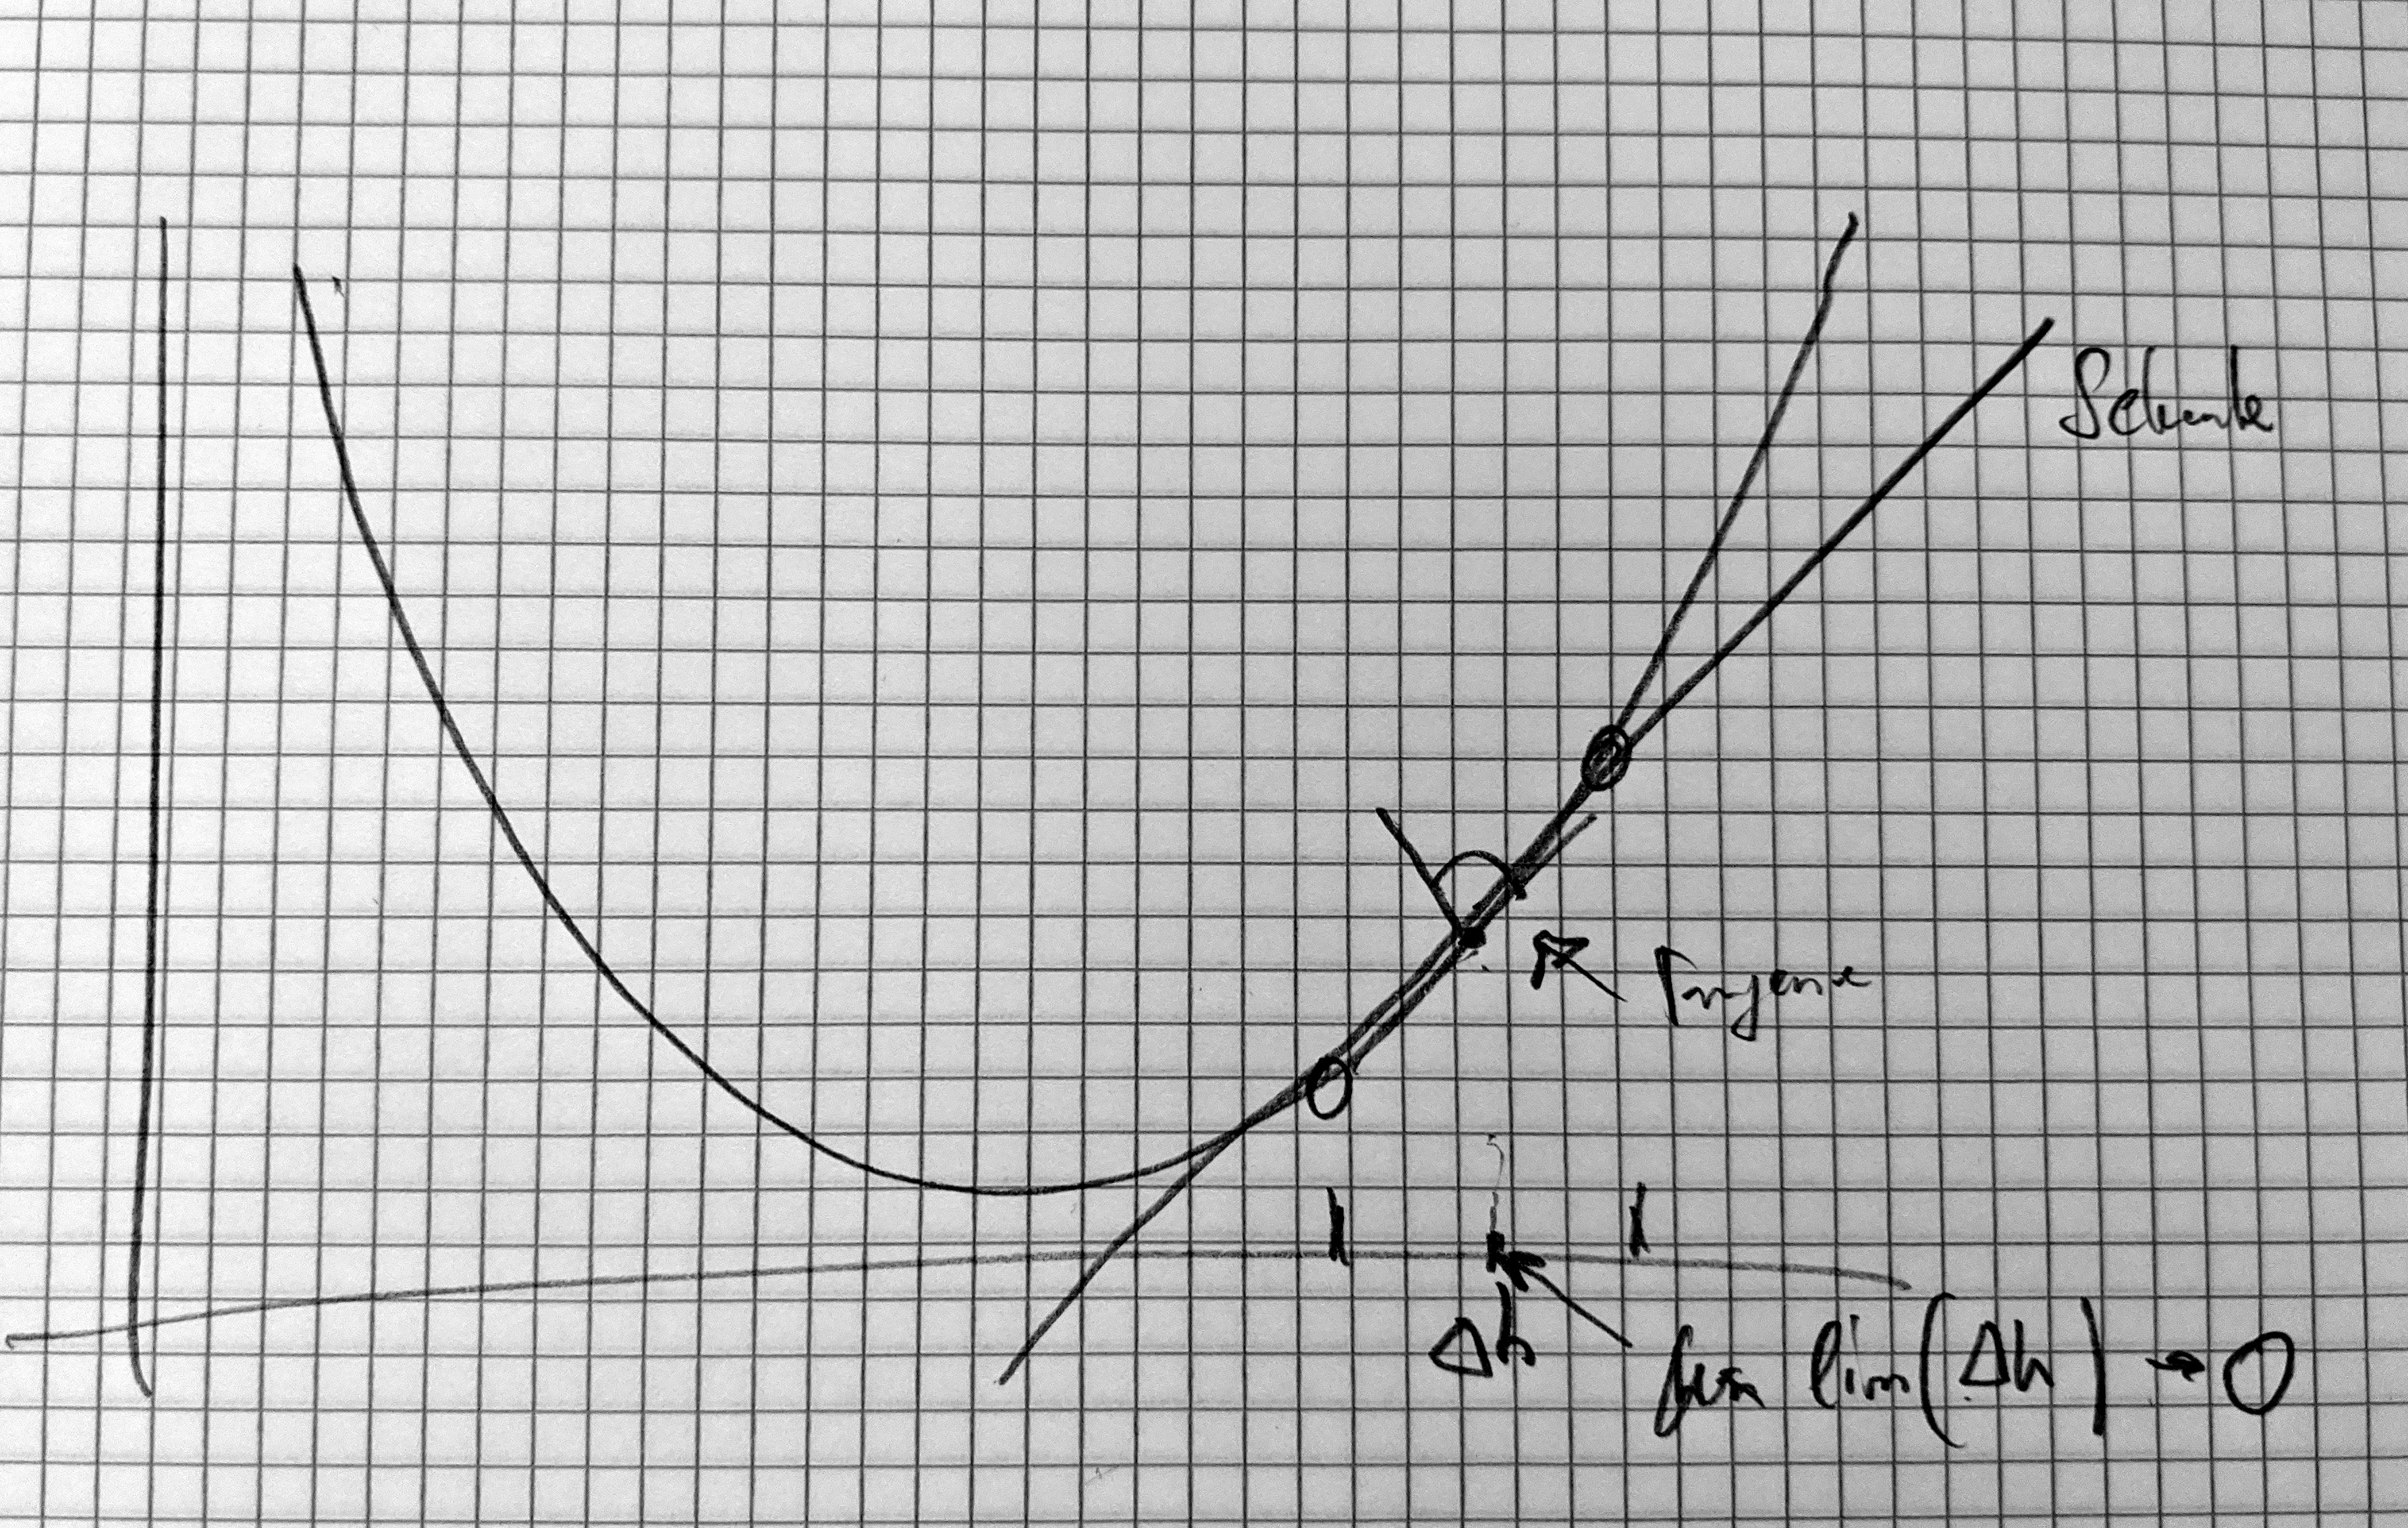
\includegraphics[width=12cm]{papers/ableitung/images/sekante_bsp.jpg}
		\caption{Testic}
		\label{ableitung:fig:ableitung_bsp}
	\end{center}
\end{figure}

\begin{equation}
\begin{split}
f'(x_0) &= \frac{f(x_0 + h) - f(x_0)}{h} \\
f'(x_0) &= \frac{f(x_0) - f(x_0 - h)}{h} \\
f'(x_0) &= \frac{f(x_0 + h) - f(x_0 - h)}{2h} \\
\end{split}
\label{ableitung:equations:differenzenquotient}
\end{equation}


% Sekante und Tangente erklären / SIN verwenden
%\begin{tikzpicture}
%\begin{axis}[
%xlabel=$x$,
%ylabel={$f(x) = x^2$}
%]

%\addplot [mark=none] {x^2};
%\end{axis}
%\end{tikzpicture}

Diese Methode ist limitiert auf die erste Ableitung und zwei Stützstellen, jeweils im Abstand von $h$.

\subsection{Taylor Methode}

Mithilfe der Taylor Reihe lässt sich jede beliebige Funktion $f(x)$ approxmieren. Dies machen wir uns für die Herleitung zu Nutze.

\begin{equation}
f(x) = f(a)+{\frac {f'(a)}{1!}}(x-a)+{\frac {f''(a)}{2!}}(x-a)^{2}+{\frac {f'''(a)}{3!}}(x-a)^{3}+\cdots
\label{ableitung:eqn:taylorseries}
\end{equation}

Für die n-te Ableitung benötigen wir mind. n-Sützstellen.
Die Begründung ist, dass wir ein Polynom suchen, welches mindestens n-mal Ableitbar ist und dies benötigt den Grad n. Die Bestimmung des Polynoms kann mittels Lagrange Methode oder eines Polynom-fittings vollzogen werden.
Die Stützstellen sollen alle in einem gleichmässigen Abstand $h$ uniform verteilt werden.
Daraus resultiert folgende Gleichung für unsere Approximation.

\begin{equation}
\frac{\delta^{4} f}{\delta x^4} \approx Af(x-2h) + Bf(x-h) + Cf(x) + Df(x+h) + Ef(x+2h)
\end{equation}

Die jeweiligen Stützstellen können nun mittels Taylor-Reihe erweitert werden:

\begin{equation}
\begin{split}
Af(x-2h) \approx & Af(x) + Af'(x)(-2h) + A\frac{1}{2}f''(x)(-2h)^2+A\frac{1}{6} + f'''(x)(-2h)^3+A\frac{1}{24} + \\ 
& f''''(x)(-2h)^4 + A\frac{1}{120}f'''''(x)(-2h)^5 \\
Bf(x-h) \approx & Bf(x) + Bf'(x)(-h) + B\frac{1}{2}f''(x)(-h)^2+B\frac{1}{6} + f'''(x)(-h)^3+B\frac{1}{24} + \\ 
& f''''(x)(-h)^4 + B\frac{1}{120}f'''''(x)(-h)^5 \\
Cf(x) = & Cf(x) \\
Df(x+h) \approx & Df(x) + Df'(x)(+h) + D\frac{1}{2}f''(x)(+h)^2+D\frac{1}{6} + f'''(x)(+h)^3+D\frac{1}{24} + \\ 
& f''''(x)(+h)^4 + D\frac{1}{120}f'''''(x)(+h)^5 \\
Ef(x+2h) \approx & Ef(x) + Df'(x)(+2h) + E\frac{1}{2}f''(x)(+2h)^2+E\frac{1}{6} + f'''(x)(+2h)^3+E\frac{1}{24} + \\ 
& f''''(x)(+2h)^4 + E\frac{1}{120}f'''''(x)(+2h)^5
\end{split}
\end{equation}

Bei einsetzen dieser Gleichungen in die erste Gleichung (siehe oben) ist ersichtlich, dass nur die Koeffizienten der 2. Ordnung bestehen bleiben müssen und folglich 1 ergeben müssen. Der Rest sollte durch Auslöschung verschwinden. Der Einfachheit halber können die Terme nach Ableitungsgrad sortiert werden:

%\begin{equation}
%\begin{split}
%f(x) \cdot (A + B + C + D + E) & = 0 \\
%\frac{1}{2} f'(x)(h) \cdot (-2A - B + D + 2E) &= \frac{2}{h}\\
%\frac{1}{6} f''(x)(h^2) \cdot (4A + B + D + 4E) &= 0 \\
%\frac{1}{24} f''''(x)(h^3) \cdot (-8A - B + D + 8E) &= 0 \\
%\frac{1}{120} f'''''(x)(h^4) \cdot (16A + B + D + 16E) &= 0 
%\end{split}
%\end{equation}

\begin{equation}
\begin{linsys}{6}
f(x)                        \cdot(&&  A&+&B&+&C&+&D&+&  E)&=&0 \\
\frac{1}{2} f'(x)(h)        \cdot(&&-2A&-&B& & &+&D&+& 2E)&=&\frac{2}{h}\\
\frac{1}{6} f''(x)(h^2)     \cdot(&&14A&+&B& & &+&D&+& 4E)&=&0 \\
\frac{1}{24} f''''(x)(h^3)  \cdot(&&-8A&-&B& & &+&D&+& 8E)&=&0 \\
\frac{1}{120} f'''''(x)(h^4)\cdot(&&16A&+&B& & &+&D&+&16E)&=&0 
\end{linsys}
\end{equation}

Dies lässt sich auch in Matrix Form wie folgt schreiben:
\begin{align}
\begin{bmatrix}
1 & 1 & 1 & 1 & 1 \\
-2 & -1 & 0 & 1 & 2 \\
4 & 1 & 0 & 1 & 4 \\
-8 & -1 & 0 & 1 & 8 \\
16 & 1 & 0 & 1 & 16 \\
\end{bmatrix}
\cdot
\begin{bmatrix}
A \\
B \\
C \\
D \\
E \\
\end{bmatrix}
= \frac{1}{h} 
\begin{bmatrix}
0 \\
2 \\
0 \\
0 \\
0 \\
\end{bmatrix}
\end{align}

Da die Matrix invertierbar ist lässt sich die Gleichung wie folgt umformen:

\begin{align}
\begin{bmatrix}
A \\
B \\
C \\
D \\
E \\
\end{bmatrix}
=
\frac{1}{h}
\begin{bmatrix}
1 & 1 & 1 & 1 & 1 \\
-2 & -1 & 0 & 1 & 2 \\
4 & 1 & 0 & 1 & 4 \\
-8 & -1 & 0 & 1 & 8 \\
16 & 1 & 0 & 1 & 16 \\
\end{bmatrix}^{-1}
\begin{bmatrix}
0 \\
2 \\
0 \\
0 \\
0 \\
\end{bmatrix}
=
\frac{1}{h}
\begin{bmatrix}
\frac{1}{12} \\
\frac{-2}{3} \\
0 \\
\frac{2}{3} \\
\frac{1}{12} \\
\end{bmatrix}
\end{align}
Dies ergibt für die 1. Ableitung mit 5 Stützstellen folgende Annäherung:
\begin{align}
f'(x)  \approx \frac{1f(x-2h) - 8f(x-h) + 8f(x-h) - 1f(x+2h)}{12h}
\label{ableitung:eqn:aprox_5}
\end{align}
Analog kann dies natürlich für höhere Ableitungen oder non-uniforme Stützstellen gemacht werden.
\subsubsection{Fehlerabschätzung}
Die Herleitung der finite Differenzen Methode geschieht über die Taylorreihe gemäss Gleichung \ref{ableitung:eqn_taylorseries}. Um die Approximation mit fünf Stützstellen zu erhalten wurden die Taylorpolynome bis und mit dem fünften Grad evaluiert, folglich kann man für Gleichung \ref{ableitung:eqn:aprox_5} den Fehler analog zu \ref{ableitung:eqn:error}
\begin{align}
\frac{f(x-2h) - 8f(x-h) + 8f(x-h) - f(x+2h)}{12h} = f'(x) - \frac{1}{30} f^{(5)} (x)h^{4}+R_n(x)
\label{ableitung:eqn:error}
\end{align}
Funktionen lassen sich somit mit mehr Stützstellen genauer approximieren, da der Rest $R$ mit steigender Taylor-Ordnung kleiner wird. Wenn aber die Terme höherer Ordnung schneller anwachsen als die Fakultät, so ist die Approximation nicht genau.
\subsection{Beispiele}
Es wurden wurden zwei Beispiele gesucht, welche spezielle Eigenschaften haben um zu verdeutlichen wie eine Approximation gut funktioniert und wie sie weniger gut funktioniert. Es existieren somit 2 Arten von Funktionen:
% TBD
%\begin{itemize}
%	\item {Funktionen mit verschwindendem Rest: \\
%		$\sin{x}$}
%	\item{Funktionen mit wachsendem Rest: \\
%		$\sqrt{(1-x^2)}}$}
%\end{itemize}
\label{ableitung:subsection:bonorum}

